% helloTex.m4  
%
%   An m4 file to package source files for submission.
%  After using m4 on this file, a single file will
%  be generated with the contents of the included files
%  (hello.h, testHello.c, and hello.c).
%
%  To generate a file for typesetting:
%
%   m4 helloTex.m4 > NameSrc.tex
%
%  This resulting file can be typeset if desired.

\documentclass[12pt]{article}

%\usepackage[fancybox]
%\usepackage{color}  % old
\usepackage{graphicx}
\usepackage[usenames]{color}
\usepackage[margin=1in]{geometry}
\definecolor{light-gray}{gray}{0.65}

\AddToHook{cmd/section/before}{\newpage}

\begin{document}

\section{Programming Log}

\noindent\textbf{11/16/23}

I spent 1 hour installing GLUT and getting basic OpenGL programs to compile.
When trying to compile and link via one call of gcc, I repeatedly got linking errors,
so I set up a basic makefile for ease of development.

I then spent about 30 minutes designing the program.

I then spent about 3 hours writing the program. The largest difficulty encountered was with the
Rubik's cube. Matrix multiplication was not happening in the order I expected it to happen,
and it took me some time to figure out why my rotations were not working.


\section{Program Design}

\begin{verbatim}
m4_include(`programDesign.txt')
\end{verbatim}

\section{Source Code}

\subsection{main.c}
\begin{verbatim}
m4_include(`main.c')
\end{verbatim}

\subsection{data.h}
\begin{verbatim}
m4_include(`data.h')
\end{verbatim}
\subsection{data.c}
\begin{verbatim}
m4_include(`data.c')
\end{verbatim}

\subsection{makefile}
\begin{verbatim}
m4_include(`makefile')
\end{verbatim}

\section{Output}

\subsection{The 2D function, plotted as points:}
\noindent 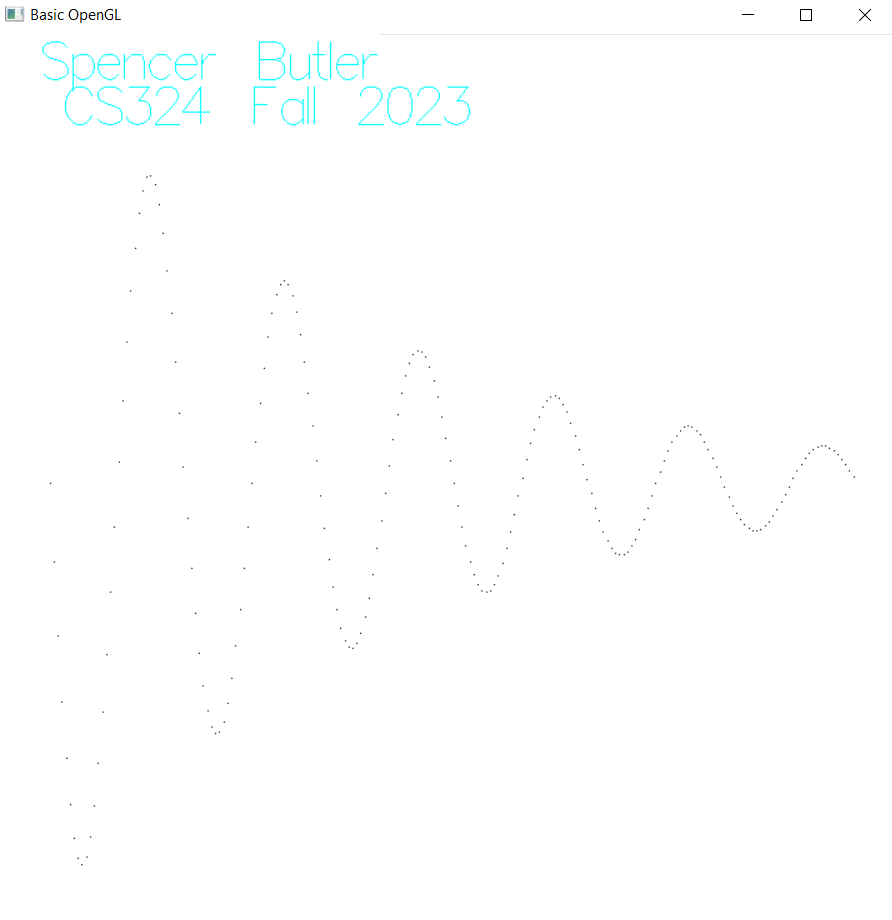
\includegraphics{screens/points}
\subsection{The 2D function, plotted as lines:}
\noindent 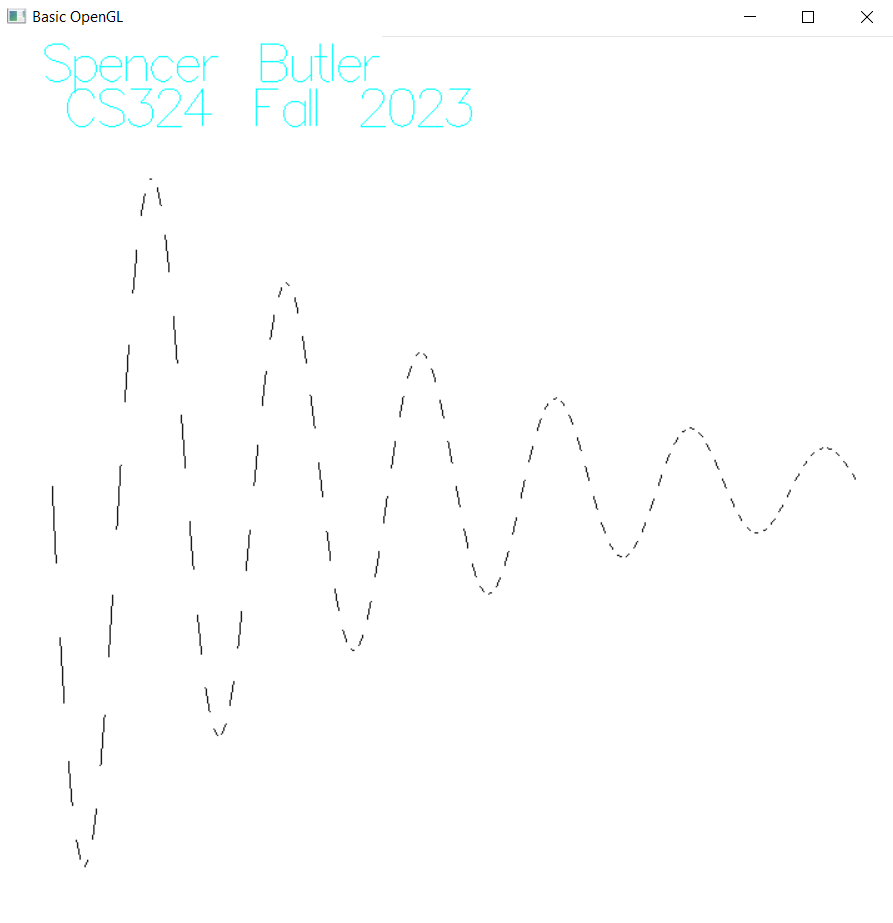
\includegraphics{screens/lines}
\subsection{The 3D function, plotted via wireframe triangles:}
\noindent 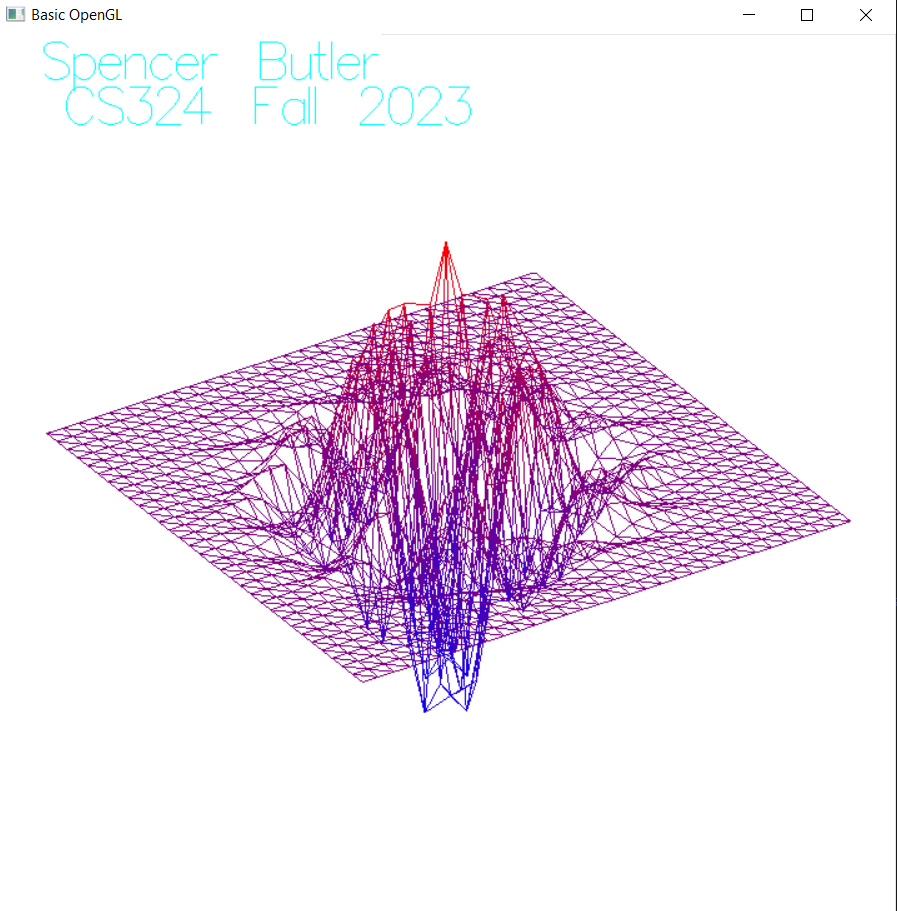
\includegraphics{screens/tris}
\subsection{All 4 ways of plotting the 3D function:}
\noindent 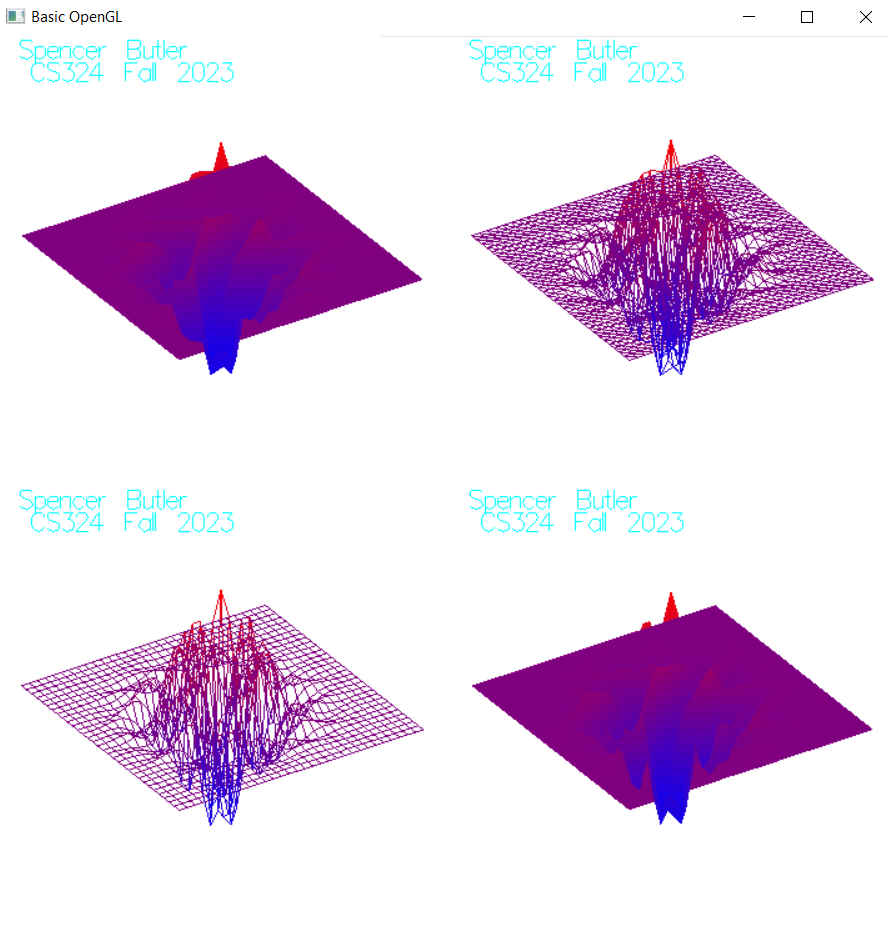
\includegraphics{screens/quadrants}
\subsection{Rubik's Cube without gaps:}
\noindent 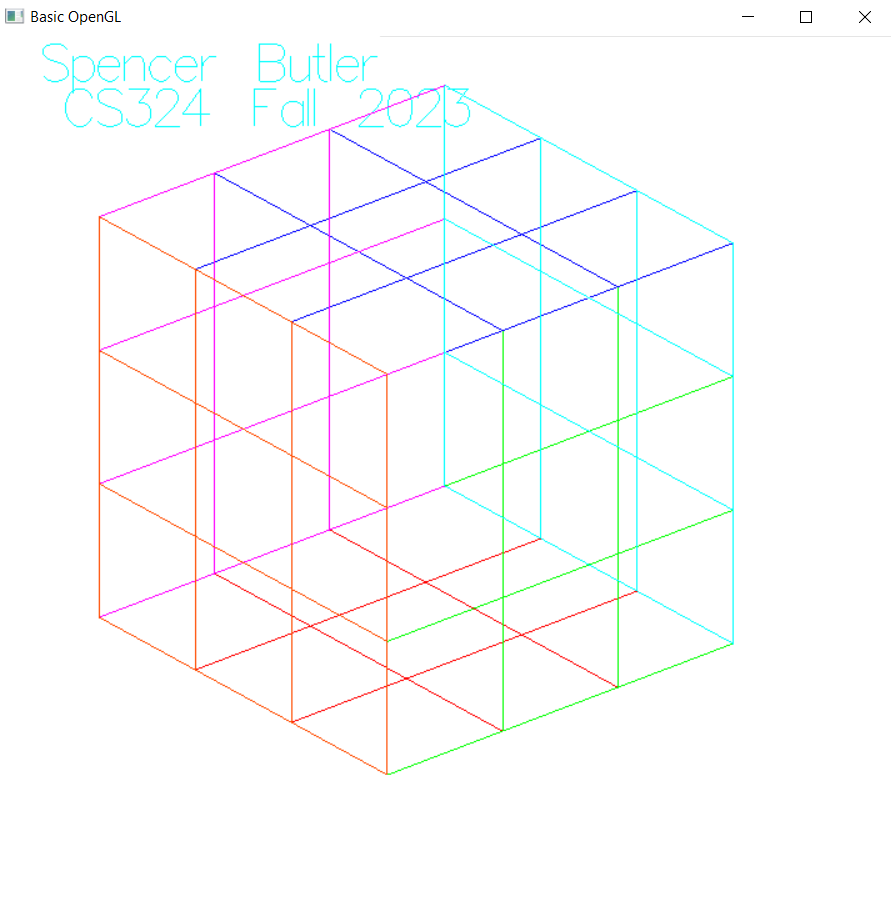
\includegraphics{screens/cube}
\subsection{Rubik's Cube with gaps:}
\noindent 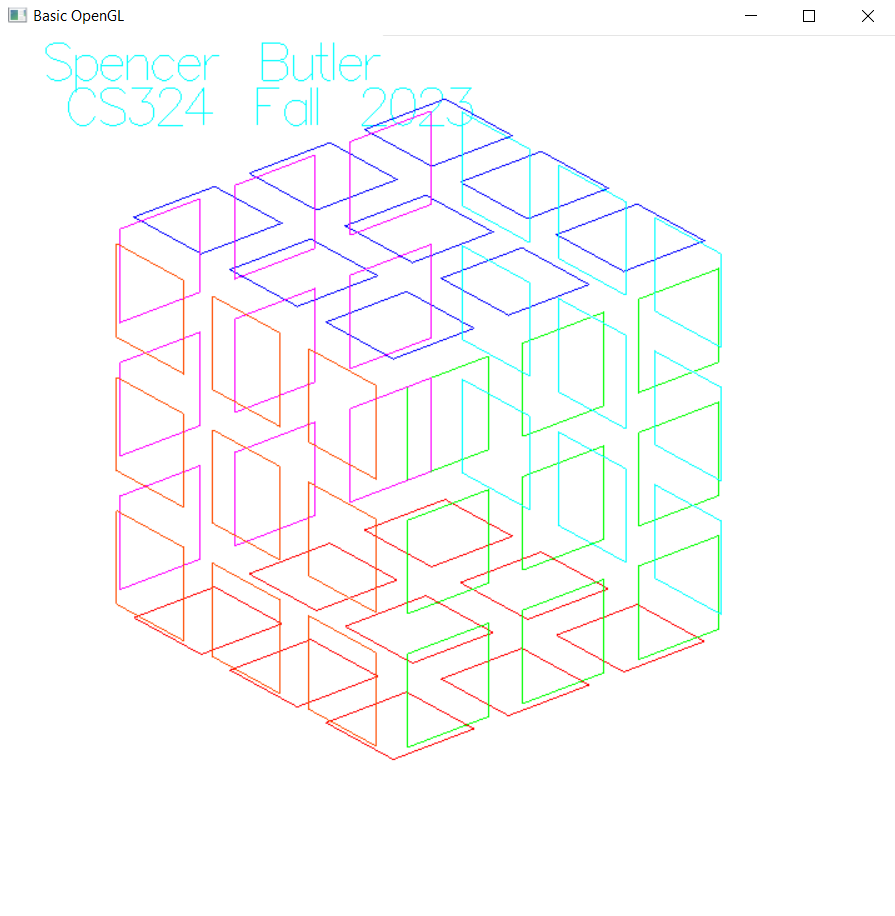
\includegraphics{screens/gaps}
\subsection{8000 cubes, with gaps:}
\noindent 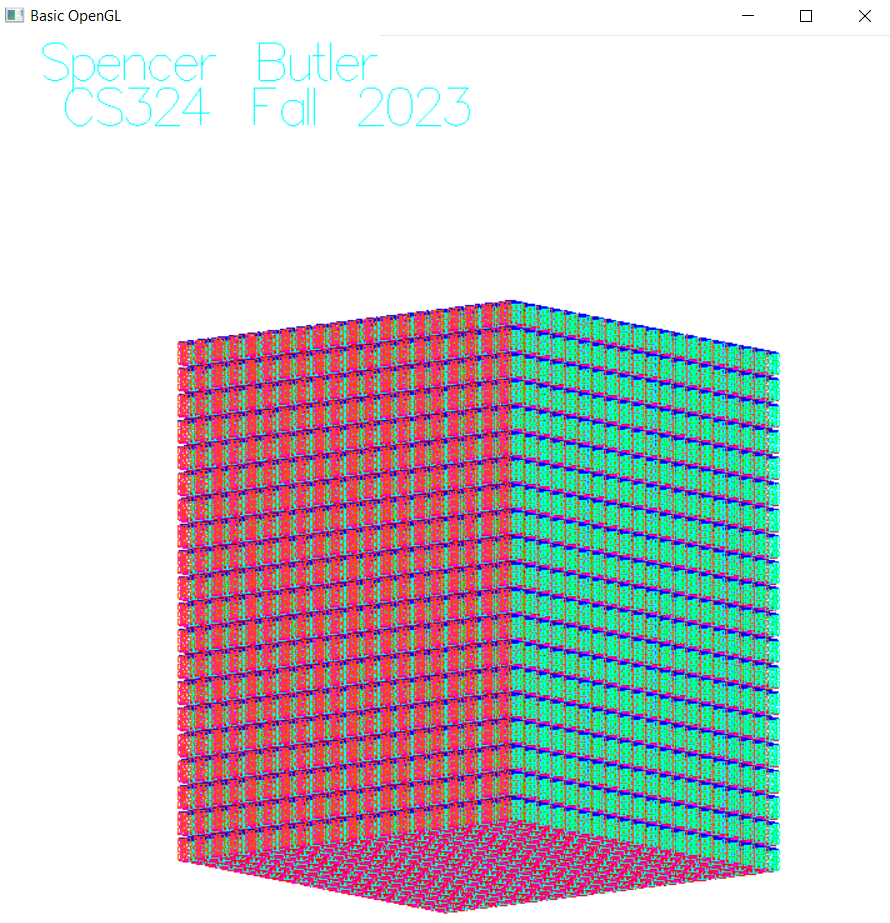
\includegraphics{screens/cubes}


\end{document}

